\documentclass[12pt,twoside]{book}
%\usepackage{elocalloc} % http://tex.stackexchange.com/questions/38607/no-room-for-a-new-dimen
\setlength{\parindent}{0em}

\hyphenpenalty=5000
\tolerance=1000

\pdfpageheight 11in
\pdfpagewidth 8.5in

\setlength{\textwidth}{6.5in}
\setlength\fboxsep{0pt}
\setlength\fboxrule{0.5pt}

\usepackage[usenames]{color}
\usepackage[titletoc]{appendix}
\usepackage{amsfonts,
            amsmath,
            amssymb,
            array,
            caption,
            enumerate,
            enumitem,
            fancyhdr,
            fourier,
            graphicx,
            hologo,
            imakeidx,   % makeidx doesn't work with xelatex for some reason
            listings,
            longtable,
            lmodern,
            minitoc,
            multicol,
            newfloat,
            parskip,
            pdfpages,
            sectsty,
            tabularx,
            tabulary,
            tcolorbox,
            tikz,
            tikz-qtree,
            ulem,
            url,
            wrapfig,
            xtab
}
\usepackage[chapter]{minted}
\usepackage[colorlinks=true,linkcolor=blue!80,urlcolor=blue!80]{hyperref}
\hypersetup{
    colorlinks=true,
    linkcolor=blue,
    filecolor=magenta,
    urlcolor=cyan,
}
\usepackage[cc]{titlepic}
\renewcommand{\mtifont}{\large\sffamily}
\renewcommand{\mtcfont}{\small\sffamily}
\renewcommand{\mtcSfont}{\small\sffamily}
\renewcommand{\mtcSSfont}{\small\sffamily}
\renewcommand{\mtcSSSfont}{\small\sffamily}
\urlstyle{same}

\partfont{\color{mLightBrown}}
\chapterfont{\color{mLightBrown}}

\usepackage[T1]{fontenc}
\usepackage{fontspec}
\setsansfont[Mapping=tex-text]{Fira Sans}
\setmonofont{FiraCode-Regular}
\usepackage[mathrm=sym]{unicode-math}
\setmathfont{Fira Math}
\renewcommand{\familydefault}{\sfdefault}

%\usepackage{cleveref} % must be loaded after hyperref

\setminted[python]{%
    bgcolor=black!5,
    fontsize=\small,
    frame=none,
    framesep=2mm,
    linenos
}
\tcbuselibrary{listings,minted}

\newtcblisting[list inside=mypy,auto counter,number within=chapter]{py}[2]{%
    colback=black!5, 
    colframe=mDarkGreen,
    coltitle=mLightBrown,
    listing only,
    sharp corners=downhill,
    minted language=python,
    minted options={numbersep=2mm},
    title=Code Example \thetcbcounter: #1,
    label=lst:#2
    %addtolol
}

\newtcolorbox[%
    auto counter,
    number within=chapter,
    blend into=figures,
    number freestyle={\noexpand\thechapter.\noexpand\arabic{\tcbcounter}}
]{myfigure}[2][]{%
    float=htb,
    capture=hbox,
    blend before title=colon hang,
    title={#2},
    label={#2},
    every float=\centering,
    #1,
    sharp corners=downhill,
    colback=white,
    colframe=mDarkGreen,
    coltitle=mLightBrown,
    %colbacktitle=blue!30!black
}

\newtcolorbox[%
]{note}[2][]{%
    before title={\textbf{Important Note: }},
    float=htb,
    blend before title=colon hang,
    title={\textbf{#2}},
    every float=\centering,
    #1,
    sharp corners=uphill,
%    colback=red!5!white,
    colback=mDarkGreen,
%    colframe=red!75!black,
    colframe=mLightBrown,
    coltitle=white,
    coltext=white
}


\usepackage[explicit]{titlesec}

\definecolor{mLightBrown}{HTML}{EB811B}
\definecolor{mLightGreen}{HTML}{14B03D}
\definecolor{mDarkGreen}{HTML}{27363A}

\makeatletter
\renewcommand{\@chapapp}{Day}
\makeatother

\usepackage[lmargin=1.5in,rmargin=0.75in,tmargin=1in,bmargin=1in]{geometry}

% TikZ stuff
\usetikzlibrary{arrows,backgrounds,calc,decorations,decorations.pathreplacing,decorations.shapes,fit,positioning,shadows,shapes,trees}



\DeclareCaptionFont{white}{\color{mLightBrown}\small}
\DeclareCaptionFormat{listing}{\colorbox{mDarkGreen}{\parbox{\textwidth}{\vspace{1mm}~~#1#2#3\vspace{1mm}}}}
\captionsetup[listing]{format=listing,labelfont=white,textfont=white}

% Define block styles
\tikzstyle{decision} = [diamond, draw, fill=blue!20,
    text width=4.5em, text badly centered, node distance=3cm, inner sep=0pt]
\tikzstyle{block} = [rectangle, draw, fill=blue!20,
    text width=10em, text centered, rounded corners, minimum height=4em]
\tikzstyle{cloud} = [draw, ellipse,fill=red!20, node distance=3cm,
    minimum height=2em]

\tikzstyle{merge_1} = [rectangle, draw, fill=blue!20,
    text width=12em, text centered, rounded corners]
\tikzstyle{merge_2} = [rectangle, draw, fill=blue!20,
    text width=7em, text centered, rounded corners]
\tikzstyle{merge_3} = [rectangle, draw, fill=blue!20,
    text width=4em, text centered, rounded corners]
\tikzstyle{merge_4} = [rectangle, draw, fill=blue!20,
    text width=2em, text centered, rounded corners]

\tikzstyle{gone} = [rectangle, draw=gray, fill=gray!20,
    text width=2em, text centered, text=gray, rounded corners]
\tikzstyle{gone_3} = [rectangle, draw=gray, fill=gray!20,
    text width=4em, text centered, text=gray, rounded corners]

\tikzstyle{empty} = [rectangle, draw, fill=blue!20,
    text width=1em, rounded corners]
\tikzstyle{emptyleaf} = [rectangle, draw, fill=green!20,
    text width=1em, rounded corners]

\tikzstyle{blank} = [rectangle]

\tikzstyle{2node} = [circle, draw, fill=blue!20,
    text width=0.3cm, text centered]
\tikzstyle{3node} = [ellipse, draw, fill=blue!20,
    text width=1cm, text centered]
\tikzstyle{new2node} = [circle, draw, fill=red!20,
    text width=0.3cm, text centered]
\tikzstyle{new3node} = [ellipse, draw, fill=red!20,
    text width=1cm, text centered]

\tikzstyle{btree} = [rectangle, draw, fill=blue!20, text centered]

\tikzstyle{line} = [draw, -latex']
\tikzstyle{background}=[rectangle, %dashed,
                        draw=blue,
                        fill=green!30,
                        inner sep=0.3cm,
                        rounded corners=5mm]


\pagestyle{empty}

\title{{\color{mLightBrown}\textbf{CSC 104 Lecture Notes}}\\}
\author{Prof. Christopher R. Merlo\\
Nassau Community College\\
\texttt{cmerlo@ncc.edu}\\
\url{http://www.matcmp.ncc.edu/~cmerlo/}
%/date{}
}
\titlepic{
\includegraphics[width=0.25\textwidth]{NCCMasterCPrint}}

% Itemize
\newcommand{\bi}{\begin{itemize}}
\newcommand{\ei}{\end{itemize}}
\newcommand{\be}{\begin{enumerate}}
\newcommand{\ee}{\end{enumerate}}
\newcommand{\bmu}{\begin{multicols}}
\newcommand{\emu}{\end{multicols}}

\makeindex
\begin{document}

\frontmatter

\let\stdsection\section

\newcommand{\code}[1]{\textcolor{mLightBrown}{\textsf{#1}}}
\newcommand{\prop}[2]{\label{prop:#1}\textcolor{mLightBrown}{\textsf{\textbf{Proposition #1:}}} \textit{#2}}
\newcommand{\qed}{~\hfill\textcolor{mLightBrown}{$\blacksquare$}}

\renewcommand{\labelitemi}{\textcolor{mLightBrown}{$\bullet$}}
\renewcommand{\labelitemii}{\textcolor{mLightBrown}{$\bullet$}}
\renewcommand{\labelenumi}{\textcolor{mLightBrown}{\theenumi.}}

\pagenumbering{roman}
\maketitle

\chapter{Copyright}

These lecture notes are \copyright~2019 Christopher R. Merlo.

This work is licensed under the Creative Commons Attribution-ShareAlike 4.0 International License. To view a copy of this license, visit \url{http://creativecommons.org/licenses/by-sa/4.0/} or send a letter to Creative Commons, PO Box 1866, Mountain View, CA 94042, USA.

\vfill\vfill

\begin{center}

\includegraphics[scale=0.85]{cc.logo.eps}

\includegraphics{by.eps}

\includegraphics{sa.eps}
\end{center}

\vfill


\dominitoc
\tableofcontents

\cleardoublepage
\addcontentsline{toc}{chapter}{List of Figures}
\listoffigures

\SetupFloatingEnvironment{listing}{name=Code Example}
\SetupFloatingEnvironment{listing}{listname=List of Code Examples}
\renewcommand{\listoflistingscaption}{List of Code Examples}

%\listoflistings
\tcblistof[\chapter*]{mypy}{List of Code Examples}
\addcontentsline{toc}{chapter}{List of Code Examples}

\cleardoublepage
\addcontentsline{toc}{chapter}{List of Tables}
\listoftables

\cleardoublepage

% !TEX root = CSC104LectureNotes.tex

\chapter{About These Notes}

\section*{Welcome Future Programmer!}

Hello!  Thank you and congratulations for choosing to study programing and problem solving at Nassau Community College!  Computers are ubiquitous in our society, and so a knowledge of how they work is very important for the educated person in the 21st century.  This course will provide a unique opportunity for you to discover how computers work, by telling them what to do!

While this course will not make you an expert programmer, learning the basics of programming -- and, perhaps just as importantly, learning how programmers think -- will give you the insights you need in understand what drives our economy, our culture, our technology, and virtually every other facet of our lives.  Even a cursory understanding of programming and of programmers will make you a better physicist, or accountant, or elementary school teacher.

\section*{How to Use This Document}

This document is meant to introduce you to the topics that you will be covering each day in class.  It is recommended that you read each day's notes \textbf{\textit{before}} coming to class.  The discussions you have in class are not meant to introduce you to these topics, but to \textbf{\textit{reinforce}} the topics.  The best strategy for succeeding in this class is to avoid surprises!  Arm yourself with as much information as possible \textit{before} attending class, and then capitalize on your new knowledge after class by \textit{practicing} what you've learned.

\subsection*{Ethical Behavior}

As Stan Lee taught us through his character Spider-Man, with great power comes great responsibility.  As the world's activities become increasingly electronic, and increasingly interconnected, we programmers must do our part to ensure the rights -- including the right to privacy -- of those whose lives our work will affect.  The ethics of programming will be discussed at various points in these notes and during the course.

To that end, we NCC Computer Science and Information Technology faculty subscribe to the \href{https://www.acm.org/code-of-ethics}{Code of Ethics} published by the \href{https://www.acm.org/}{Association for Computing Machinery}, and we will refer to this Code from time to time.

\section*{How This Document Was Created}

The tools used to create this document include:

\bi
    \item The \LaTeX{} document typesetting system (\url{https://www.latex-project.org/})
    \bi
        \item The \hologo{XeLaTeX} (\url{http://xetex.sourceforge.net/}) typesetting extension
    \ei
    \item Mozilla Project's Fira Type Family (\url{https://github.com/mozilla/Fira})
    \item VS Code (\url{https://code.visualstudio.com/})
    \bi
        \item James Yu's LaTeX Workshop extension (\url{https://marketplace.visualstudio.com/items?itemName=James-Yu.latex-workshop})
    \ei
    \item Green Mountain Coffee Roasters Colombia Select (\url{http://www.gmcr.com/})
\ei
% !TEX root = CSC104LectureNotes.tex

\chapter{Acknowledgments}

My sincere thanks to my colleagues in the Department of Mathematics, Computer Science, and Information Technology, who encouraged me to apply for a sabbatical, and who taught my classes in my absence, so that I could prepare this material.  In particular, thanks to the members of the CSC 104 course committee, who helped guide me during some critical decision making.  Thanks also to the Nassau Community College Federation of Teachers' Sabbatical Committee, for their hard work to ensure that professors like me get the opportunity to do this kind of work.

\newpage
\pagenumbering{arabic}

\pagestyle{fancy}

% Even page: chapter on right
% Odd page: section on left

\fancyhead[RE]{\color{mLightBrown}\textbf{\small\nouppercase\leftmark}}
\fancyhead[RO]{\color{mLightBrown}\textbf{\thepage}}
\fancyhead[LO]{\color{mLightBrown}\textbf{\small\nouppercase\rightmark}}
\fancyhead[LE]{\color{mLightBrown}\textbf{\thepage}}
\fancyfoot[C]{}

% Definitions
\newcommand{\review}{%
  \fcolorbox{reviewcolor}{red!5}{\parbox{\textwidth}{%
  \vskip10pt
  \leftskip10pt\rightskip10pt
  \textcolor{reviewcolor}{\textsf{\textbf{This is review material.}}}\\
  You should have been familiar with this upon passing CSC 130.  Be sure to go over this on your own, and ask questions in office hours if you need reinforcement.\\
}} \vspace{0.5em} }

\newcommand{\topquote}[2]{%
    {\small
    \fcolorbox{mDarkGreen}{mDarkGreen}{\parbox{\textwidth}{%
        \vskip10pt
        \leftskip10pt\rightskip10pt
        {\textcolor{mLightBrown}{#1}}\\
        {\textcolor{mLightGreen}{\textit{ -- #2}}}\\
    }}\vspace{0.5em}
}}

\newcommand{\addindex}[2]{%
    \index{#1}\textbf{\textcolor{mLightBrown}{#2}}%
}

\mainmatter

\part{Problem Solving}

\adjustmtc
\adjustmtc
\adjustmtc
\adjustmtc

% !TEX root = CSC104LectureNotes.tex

\setcounter{chapter}{0}
\chapter{Course Introduction}

\topquote{If I had an hour to solve a problem I'd spend 55 minutes thinking about the problem and 5 minutes thinking about solutions.}{Albert Einstein}

\minitoc

Welcome to {\color{mLightBrown}CSC 104: Programming Logic and Problem Solving!}  This course is intended for Information Technology majors, Computer Science majors, and anyone else who's interested in learning about computer programming and about computer programmers.

\section{Course Strategies}

Two personality traits that seem to be common to successful programmers are:
\begin{itemize}
\item Curiosity
\item Perseverance
\end{itemize}

Why is that?  Many computer programmers spend a lot of time solving problems that have never been solved before.  This often requires thinking about an old problem in a new way, and deciding not to give up.

Also, sometimes the best result is not a complete answer, but just an answer that's incrementally better than the most recent answer.  Small successes are successes, and we must accept them and celebrate them!  Sometimes programmers talk about being \textbf{productively lost} -- not quite sure which way to proceed, but at least having a good understanding of the problem one is in.

For these reasons, it is important that you \textbf{ask lots of questions}, during class, in your professor's office hours, or over electronic communication.  Every question moves the conversation, and aids in problem solving.  Even asking a ``bad'' question helps eliminate an avenue of inquiry that might not have led to success.

Related to this idea, it's important that you \textbf{answer every question} during class or on homework.  Even if your answer is wrong or incomplete, a ``bad'' answer is something you can build upon.

Make sure to \textbf{review what you've learned} after every class, and make sure everything makes sense.  Ask questions as soon as you have to, in order to get back on track.

Finally, make sure you understand your professor's policies.  \textbf{Read the syllabus} and understand your responsibilities, and what's expected of you.  Check on when things like exams are expected to happen, and add them to your calendar now.

\section{Daily Preview}

Each day, your professor will display a slide like this:
\begin{myfigure}{Typical Lecture Introduction Slide}
	%\caption
	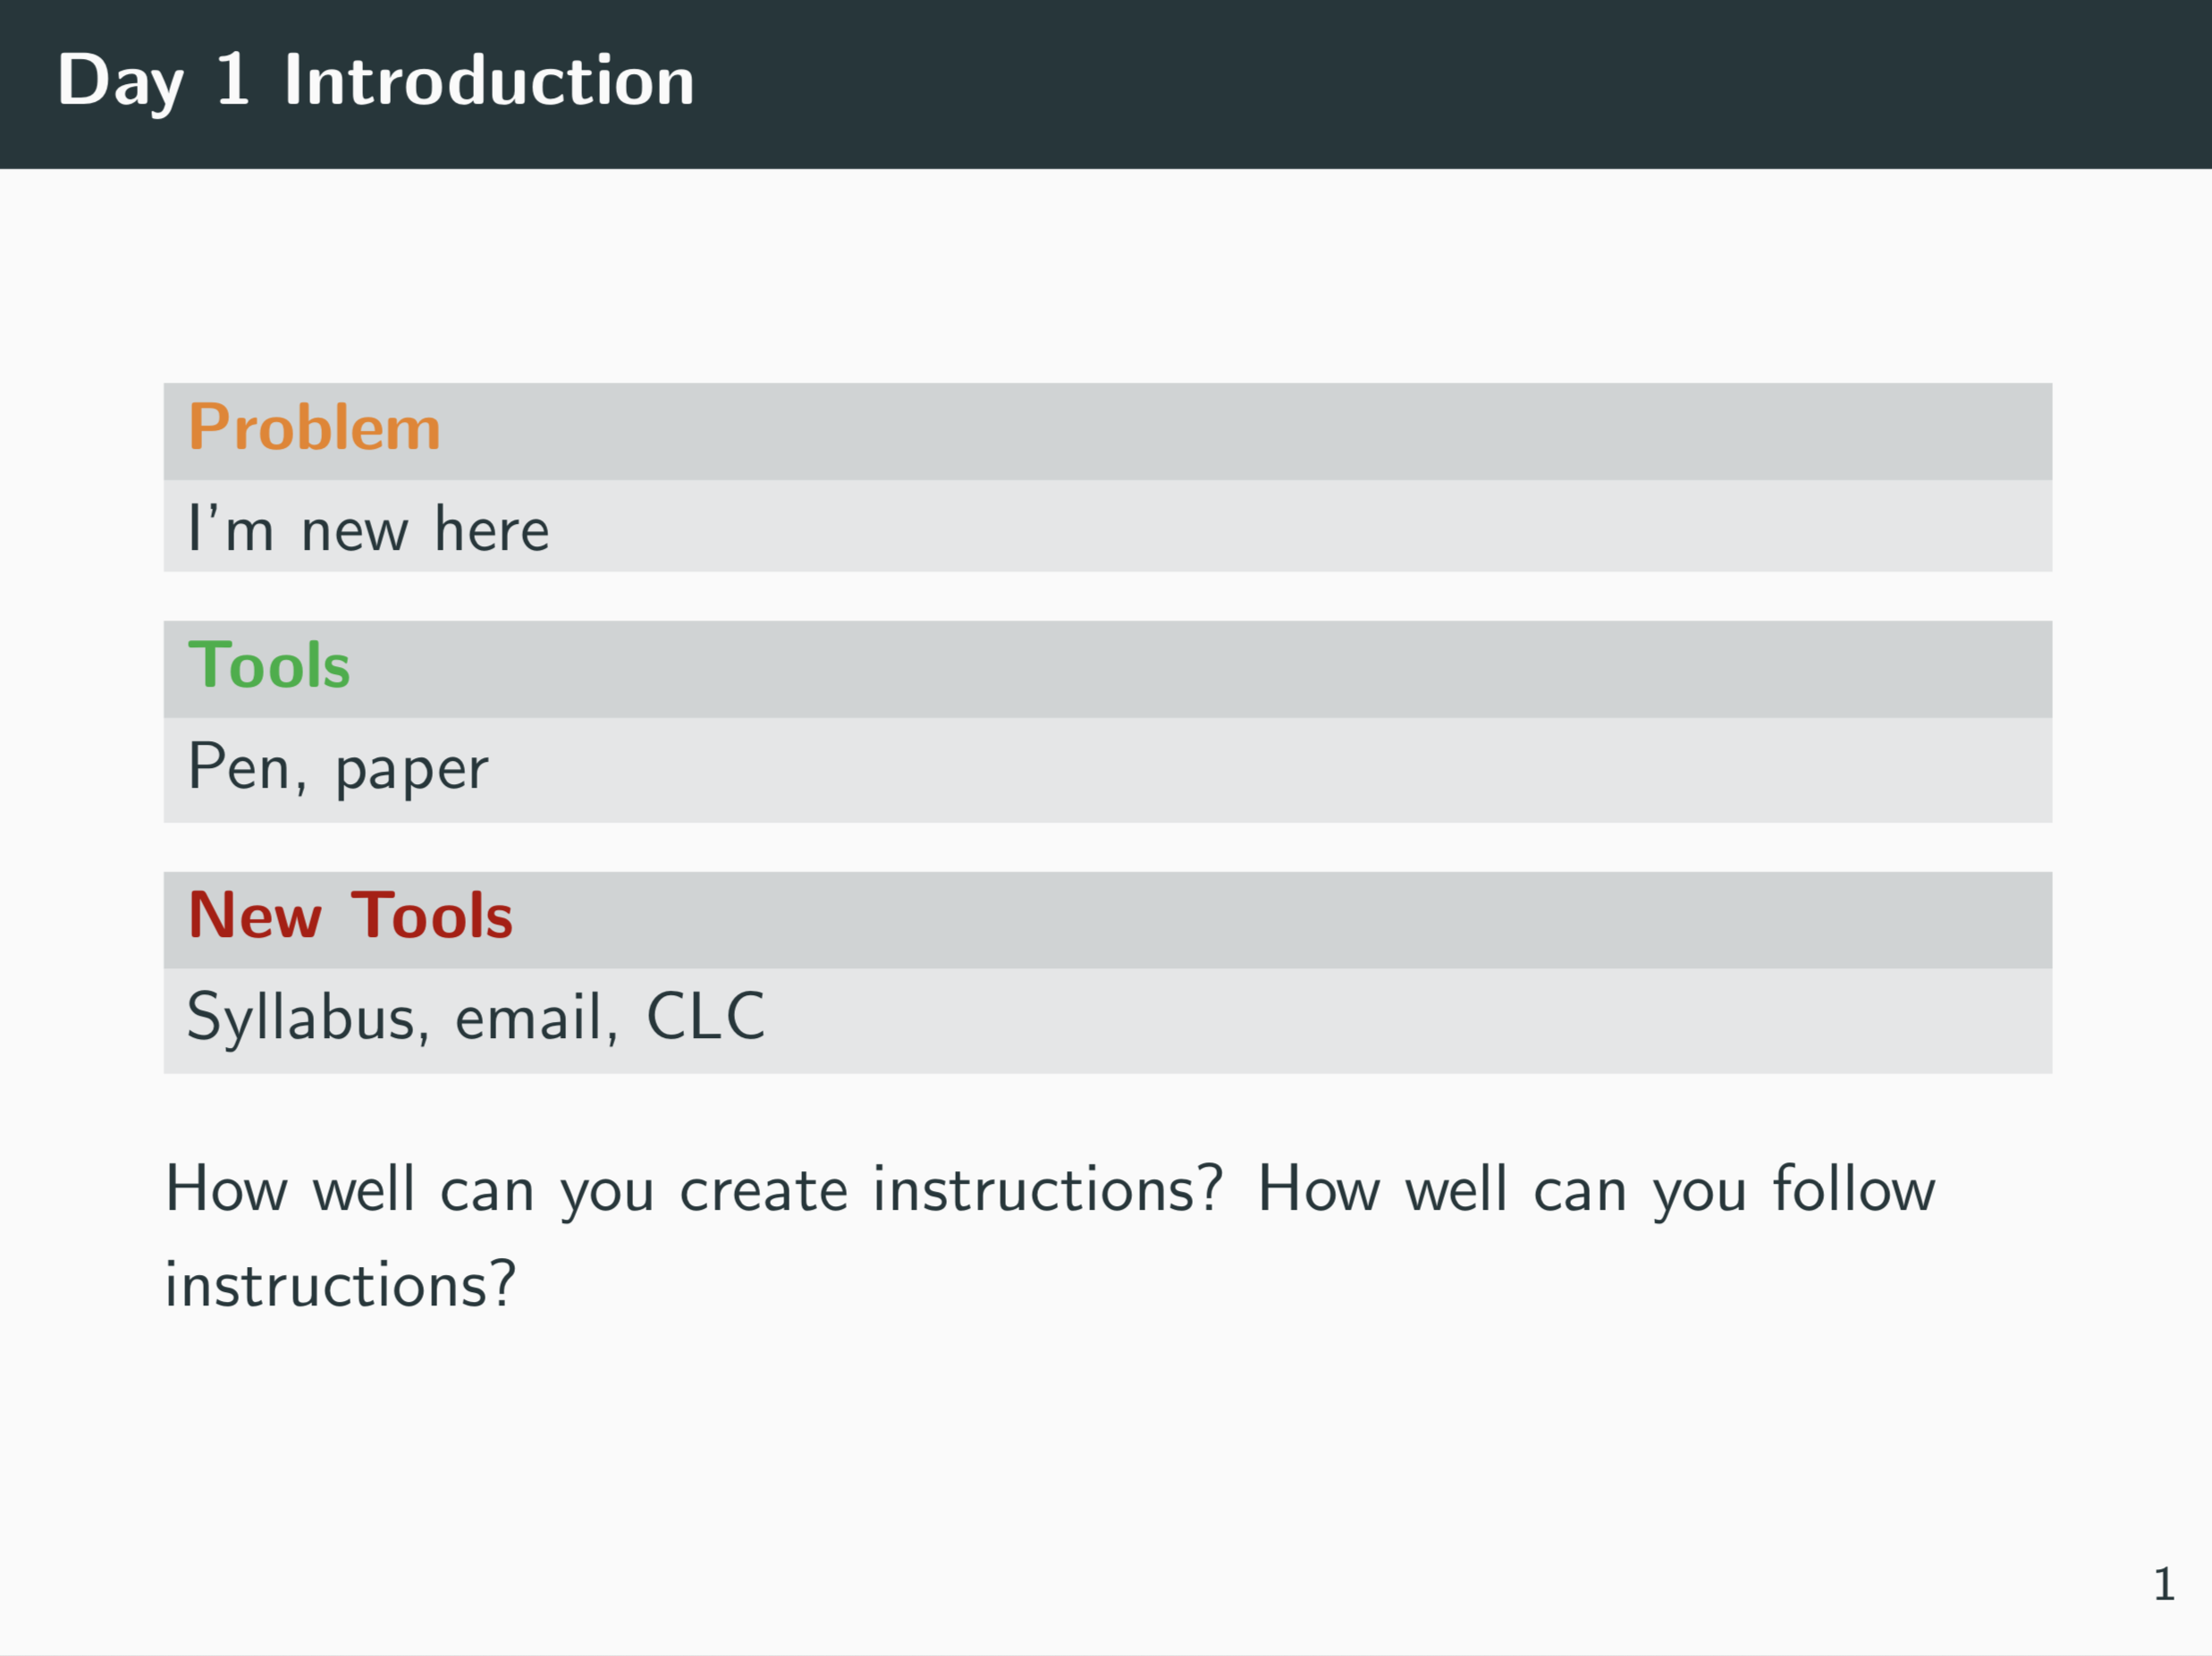
\includegraphics[scale=0.25]{day1slide}
\end{myfigure}

Understanding the day's problem, tools to be used, and new tools to be acquainted with, is a good way to get into the right mindset for the day's activities.

\section{Interview Questions}

It was once very popular for hiring officers to ask programmers to solve very difficult logic puzzles during job interviews.  These questions are no longer used so frequently, but they were popular because, it was thought, they allowed the interviewers to see how the interview subjects think about new problems.  As we work through the first part of this course, we will examine questions like this, to try to gain insight into how programmers think, and why it seems that programmers think about things in a different way than other people do.

The article that begins on Page \pageref{cnn} at the end of today's notes describes the situation well.

\section{Logo Exercise}

The best way to learn how to do anything is to do it.  Several times this semester, you will be engaging in a hands-on activity, meant to help you enhance a skill that you will be relying on throughout the rest of the course.  Today, you will learn just how difficult it can be to write directions and to follow them.

\section{Homework}

For homework, make sure you do the following things:
\begin{itemize}
\item Sign up for any web sites your professor asked you to sign up for, like the course management system, communications tools, etc.
\item Purchase access to the zyBooks textbook
\item Familiarize yourself with the location of the Computer Learning Center in B 225
\end{itemize}

\newpage
\label{cnn}
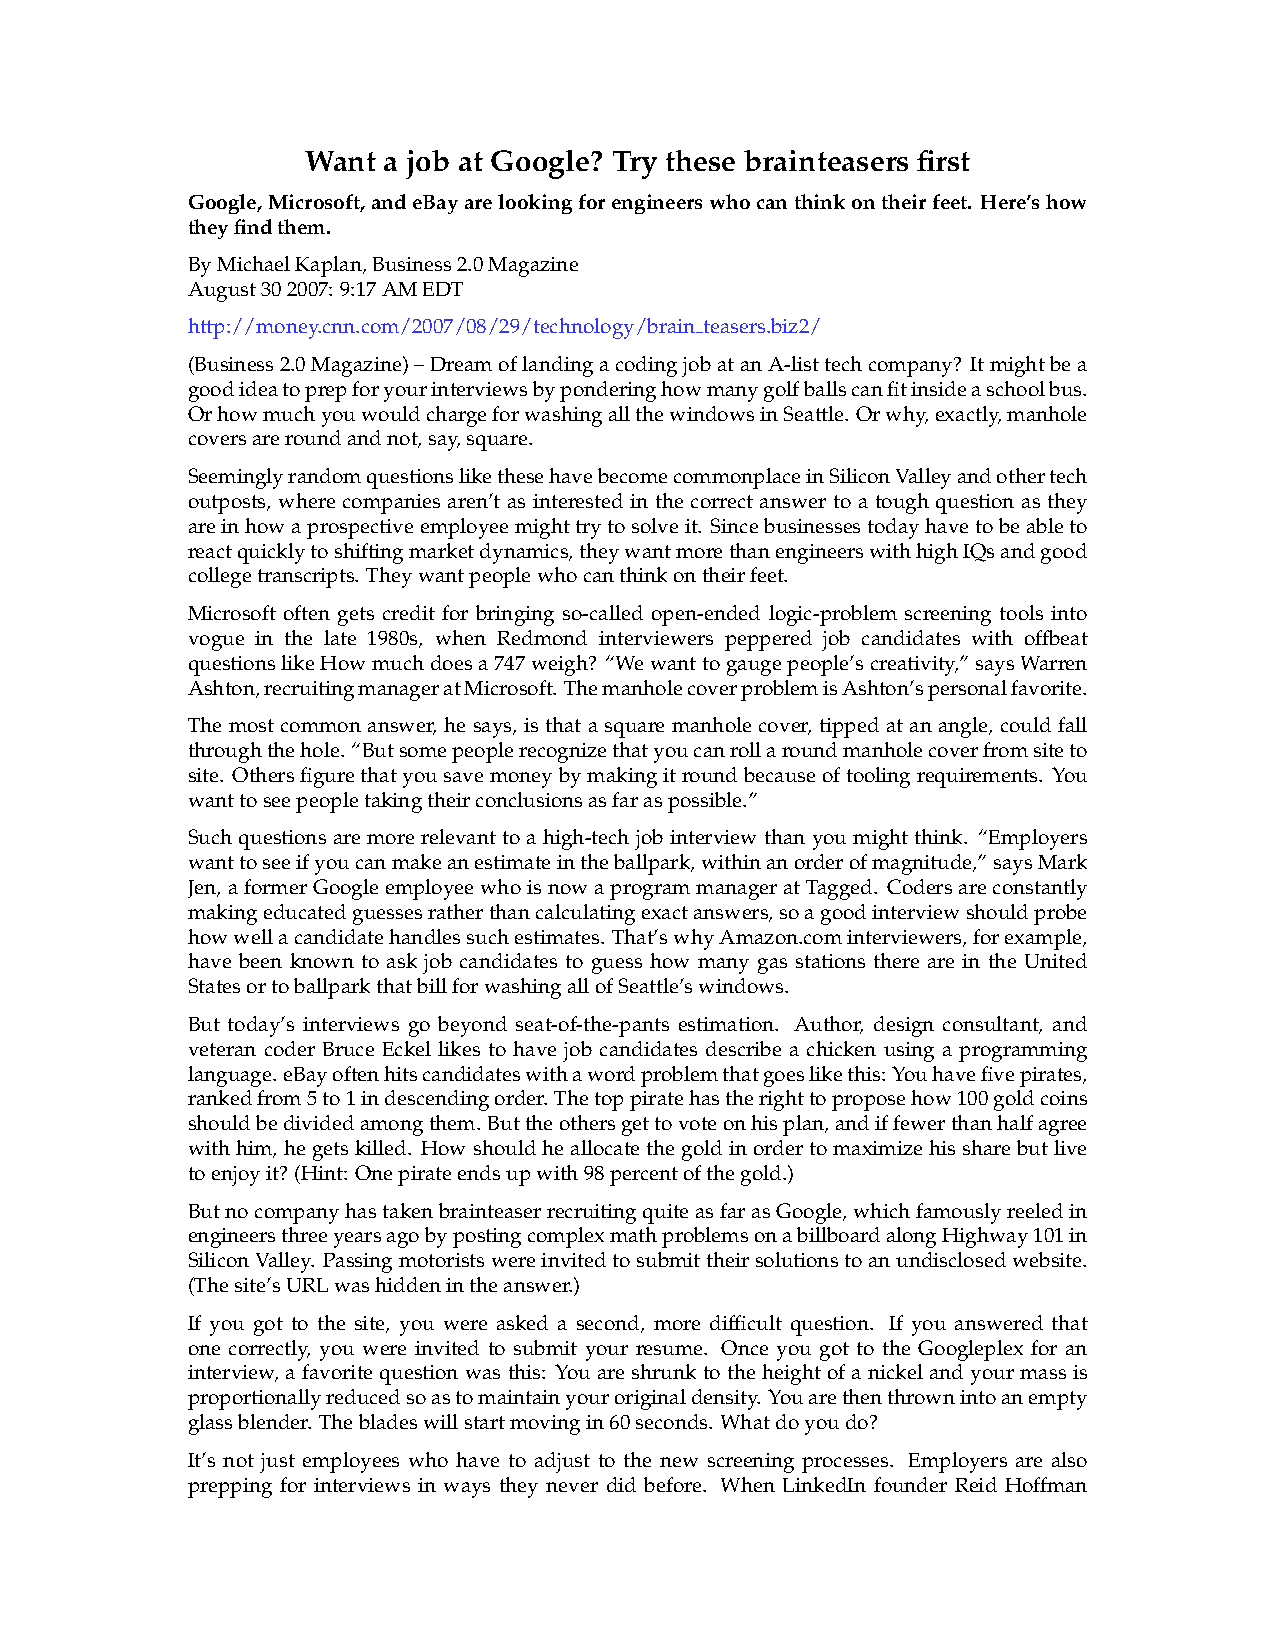
\includepdf[pages=-,pagecommand={\pagestyle{fancy}},noautoscale,scale=0.9]{day1-interview-article.pdf}

% !TEX root = CSC104LectureNotes.tex

\setcounter{chapter}{1}
\chapter{Talking Like a Programmer}
\label{day:vocabulary}

\topquote{It's all talk until the code runs.}{Ward Cunningham}

\minitoc

\section{Interview Question}

Your professor will give you a challenge regarding the crossing of a rope bridge.  Remember -- what's most important is that you make a guess, even if it isn't right.  A ``bad'' guess can help lead to the correct answer!

\section{Vocabulary}

Some people think, when they hear programmers talk, that they're speaking a foreign language.  Hopefully, today's lesson will help familiarize you with some of the jargon we use.  If you're going to do programming, it's important that you understand the spoken language that will be used, so that you can converse with the people you'll be working among.

\subsection{What Is a Computer Program?}

A \addindex{Program!Definition}{computer program} consists of a series of instructions that we humans write, using a vocabulary that the computer can understand.  When the computer \textit{executes}, or runs, our instructions, it will do so exactly as they are written, and so it's important that we write these instructions using the right language, in the right order, and without any ambiguity.

A person who is in the process of creating a program is said to be engaged in \addindex{Program!Programming}{computer programming}.  But programming isn't just the act of typing stuff on a keyboard; it also involves \textbf{testing} the program to see whether it works, and then \textbf{debugging}, or removing the problems we've programmed in.

\subsection{What Is an Algorithm?}

This leaves us with the question of what to type in.  How do we know which instructions to give to the computer?

The process of programming starts with designing an algorithm.  An \addindex{Algorithm}{algorithm} is a set of instructions that can be used repeatedly to solve a problem.  You probably have some algorithms you follow every day, like preparing breakfast or walking to class from the parking lot.  You could probably sit at home and describe to another student over the phone how to walk to the B building from where you normally park.  Some important characteristics of algorithms are that they're \textbf{repeatable} and \textbf{describable} to another person.

A programmer, then, describes an algorithm to a computer, by writing instructions in the computer's language.

\subsection{What's In a Computer?}

Most modern computers, whether on your desk or in your pocket, have these components:
\subsubsection{Central Processing Unit}
The \index{CPU|see {Central Processing Unit}}\addindex{Central Processing Unit}{central processing unit}, or \textbf{CPU}, is the part of the computer that performs all of the instructions we write.  It keeps track of what instruction needs to be performed next, and makes sure the right things show up on the screen and get stored in memory.  CPUs are frequently measured by how many billions of operations they can perform in a second, using the unit of measurement \textit{gigahertz} (GHz).

\subsubsection{Memory}
\label{sec:memory}
The computer's \addindex{Memory}{memory}, also called \textit{primary storage}, stores programs until they're ready to be run, and it also stores data and information that programs need while they run.  When you learn about \textit{variables} later, you will learn that they get stored here.

We measure the capacity of a computer's memory in \textit{gigabytes}, or how many billions of bytes it can store.  In a typical desktop computer, the memory used by programs (\textit{RAM}, or \textit{random access memory}) only works when there's a constant supply of electricity; if the computer loses power, the memory will be emptied.

\subsubsection{Drives, Disks, and Long-Term Storage}
There are many kinds of \textit{secondary storage} available for various kinds of computers.  They are frequently refered to as \addindex{Hard Drive}{hard drives} or \textit{disks}, although these terms don't apply to some of the newest choices.  Whether they use old-fashioned spinning platters or not, however, they are used to store lots of data for a long time, including when the computer is off.  Hard drives are used to store our programs when they're not in use, and our files, like term papers, saved game progress, and songs.

\subsubsection{Input and Output}
Keyboards, screens, mice, speakers, and similar devices allow us to \addindex{Input}{input} information into the computer, and allow the computer to \addindex{Output}{output} information back to us.  Computers can work just fine without these devices, but not in an interactive way.

\subsection{Kinds of Programming Errors}
\label{sec:kindsoferrors}

There are three broad categories of errors that can exist in a computer program.  The first is an error in the structure of our instructions, and the second is an error in the logic of our instructions.  (The third is an error in the execution of our instructions, but we'll talk about these kinds of errors later.)

A \addindex{Error!Syntax error}{syntax error} is an error that arises when we programmers type something that does not follow the structural rules of the programming language in which we're writing.  Consider a similar error in a natural language.  What's wrong with this English sentence?

\begin{myfigure}[label=fig:syntax-error-in-English]{A syntax error in English}
    \begin{tcolorbox}[floatplacement=h,width=\textwidth,colback=black!10]
        \centering
        \textbf{\textit{\large{This sentence no verb.}}}
    \end{tcolorbox}
\end{myfigure}

The problem there is that we broke the rules of English -- specifically, the rule that says a sentence has to have a verb.

Now consider this sentence:

\begin{myfigure}[label=fig:semantic-error-in-English]{A semantic error in English}
    \begin{tcolorbox}[floatplacement=h,width=\textwidth,colback=black!10]
        \centering
        \textbf{\textit{\large{My dog drove me to school today.}}}
    \end{tcolorbox}
\end{myfigure}

The structure of this sentence is valid.  A grammarian would have no problem with this sentence.  A logician, however, would bristle at this, because it doesn't make any sense.  The sentence in Figure \ref{fig:semantic-error-in-English} doesn't contain any syntax errors, but it does contain an error.  Specifically, this sentence has a \addindex{Error!Semantic error}{semantic error}, which is an error in the logic or meaning of a statement.

\subsection{How the Computer Reads Our Instructions}

Certainly we humans don't communicate with each other using computer programming languages, and so when we write programs, we're performing a sort of translation, or interpretation, of our algorithm into that language.  You may be surprised, however, to learn that even a programming language is not a computer's native language.  The only language the computer natively understands is numerical in nature -- instruction 1 might mean ``add these two numbers,'' and instruction 2 might mean ``compare these two numbers, and store the result over here.''  Therefore, we need a program to translate our computer programming language instructions -- which we call \addindex{Source code}{source code} -- into machine language instructions.  There are two ways this can happen.

Some languages utilize a program called a \addindex{Compiler}{compiler}, which examines all of our source code at once.  If all of the source code is free of syntax errors, the compiler will then translate the entire program to machine language code.  The code that comes from the compiler is saved on disk, and can be run multiple times without having to be compiled again.  Other languages' source code is fed into an \addindex{Interpreter}{interpreter}, which attempts to execute each instruction of a program separately.  An interpreter can run some of a program, even if there's a syntax error somewhere in the middle; however, once a syntax error is encountered, the interpreter will immediately exit.

The language we will be programming in this semester, called Python, is a compiled language, but the resulting code is not machine code.  Instead, the Python compiler creates something called \addindex{Bytecode}{bytecode}, which then must be run by an interpreter.

\section{Three Fundamental Components of a Program}
\label{sec:threekinds}

There are three basic kinds of instructions that we programmers can write when implementing our algorithms in computer code.

\subsection{Sequential Statements}

It's important for some instructions to take place in a certain order.  When you're making breakfast, you can't put your knife in the preserves jar if you haven't taken the lid off first.  \addindex{Statement!Sequential}{Sequential statements} must be typed in in the proper order when necessary.

\subsection{Selection Statements}

Did you plug in your mobile phone when you got to class today?  Why?  Is there a certain threshold of battery percentage at which you worry about it lasting through class?  We can write certain instructions for the computer to select what to do, based upon a condition.  \addindex{Statement!Selection}{Selection statements} (also known as \addindex{Statement!Conditional}{conditional statements}) allow us to allow the computer to make a decision.  We'll explore those more in a few weeks.  \index{Conditional statement|see {Statement}}

\subsection{Iteration Statements}

How was parking today?  Did you have to drive in circles around a section of the parking lot?  Any repeated action like that is called \textit{iteration} by programmers, and so an \index{Statement!Iteration|see {Loop}}\addindex{Statement!Loop}{iteration statement}, or \textit{loop}, is the kind of instruction we write when we want some task to happen over and over again.

\section{Programming Ethics}

From time to time in this course, we will discuss the responsibilities we programmers have to the people whose lives our work might affect.  The \href{https://www.acm.org/code-of-ethics}{Code of Ethics} published by the \href{https://www.acm.org/}{Association for Computing Machinery} is a resource that is widely accepted throughout the computing industry, and one to which all of us that teach Computer Science and Information Technology here at Nassau subscribe.

\subsection{General Principles}

The first part of the Code of Ethics lists a programmer's General Principles.  Our first principle is this:

\begin{tcolorbox}[width=\textwidth,colback=black!10]
Contribute to society and to human well-being, acknowledging that all people are stakeholders in computing.  [\href{https://www.acm.org/code-of-ethics#h-1.1-contribute-to-society-and-to-human-well-being,-acknowledging-that-all-people-are-stakeholders-in-computing.}{direct link}]
\end{tcolorbox}

This principle affirms our responsibility to use our talents for the benefit of society.  It is not only easy, but far too common, for people, organizations, and corporations to forget this principle and, either through mistakes or through overt acts, create software and computer systems that do not benefit society, and potentially even cause harm to people or computers.  Computers -- and, by extension, programmers -- have changed the world for the better, but we must always strive to maintain the trust that society has placed in us.

\section{Writing and Following Directions Exercise}

Your instructor is going to ask you and a partner to write some instructions, but with some restrictions.  Then we will see how you did.

\section{Homework for Day 3}

Ted and Ken, and their wives Allyson and Janie each have a favorite sport.  The sports they enjoy are running, swimming, biking, and golf.  Based upon these clues, determine whose favorite sport is which, and submit the answer for homework before Day 3 begins.  Your instructor will give you instructions for submitting your answer.
\begin{enumerate}
\item Ted hates golf.
\item Ken wouldn't run around the block if he didn't have to, and neither would his wife.
\item Each woman's sport is featured in a triathlon.
\item Allyson bought her husband a new bicycle for his birthday, to use in his favorite sport.
\end{enumerate}

% !TEX root = CSC104LectureNotes.tex

\newcommand{\mO}{\textbf{\textcolor{mLightGreen}{O}}}
\newcommand{\mX}{\textbf{\textcolor{mLightBrown}{X}}}

\setcounter{chapter}{2}
\chapter{Matrix Logic}

\topquote{Unfortunately, no one can be told what the Matrix is. You have to see it for yourself.}{Morpheus}

\minitoc

\section{What Is Matrix Logic?}

It can be hard to know how to solve a problem that has multiple elements and multiple possibilities.  Part of the transition into thinking like a programmer involves the ability to organize information and eliminate impossibilities in a systematic way.  A \addindex{Matrix}{matrix} helps us set up a one-to-one correspondence among the elements in a problem.

\section{Example Matrix Problem}

\textbf{The problem statement:} Three friends, Sarah, Natalie, and Charlotte, all had dates on Saturday night, with Nick, Matt, and Ben.  One couple went to the movies, one went to the park, and one went out to dinner.  Based on these text messages, see if you can determine who went out with whom, and where they went.

\begin{minipage}{\textwidth}
\textbf{The clues:}\\

\begin{tcolorbox}[width=\textwidth,colback=black!10]
5:45\\
Can't believe how cold it is and the grass is all wet, yuck. It's okay though, Matt gave me his coat, I think he really likes me.\\

8:34\\
Hey guys, hope you're having a better time than I am. Ben is such a bore, I don't think I'll be doing this again. xoxoxo love, Sarah oxoxox\\

9:24\\
Wow, this movie is fantastic and he's just as into it as I am. I don't think it'd ever be as fun with a geek like Matt (no offence). I don't ever want this to end. Good luck on your dates, love Natalie
\end{tcolorbox}
\end{minipage}

\textbf{The strategy:}  Did Sarah go out with Ben?  Did Natalie go to the park?  We need a system of solving this problem that helps us eliminate the combinations that couldn't have happened, so that we leave only the one solution that makes sense.

For a problem like this, the best strategy is to create a \textbf{matrix} like this:

\begin{myfigure}[label=fig:datesmatrix]{Dates Problem Matrix}
    \begin{tcolorbox}[width=\textwidth,colback=black!10]
        \begin{center}
            \begin{tabular}{r|c|c|c||c|c|c|}
                & Nick & Matt & Ben & Movies & Park & Dinner\\
                \hline\hline
                Sarah & & & & & & \\
                \hline
                Natalie & & & & & &\\
                \hline
                Charlotte & & & & & & \\
                \hline\hline
                Movies & & & \\
                \cline{1-4}
                Park & & & \\
                \cline{1-4}
                Dinner & & &\\
                \cline{1-4}
            \end{tabular}
        \end{center}
    \end{tcolorbox}
\end{myfigure}

Some of the clues in a problem like this help us match two pieces of information.  We will place a capital letter \mO{} where we have a match.  Read the first text message again.  We don't know who sent it, but we know she's in the park with Matt, so we can update the matrix like this:

\begin{tcolorbox}[width=\textwidth,colback=black!10]
    \begin{center}
        \begin{tabular}{r|c|c|c||c|c|c|}
            & Nick & Matt & Ben & Movies & Park & Dinner\\
            \hline\hline
            Sarah & & & & & & \\
            \hline
            Natalie & & & & & &\\
            \hline
            Charlotte & & & & & & \\
            \hline\hline
            Movies & & & \\
            \cline{1-4}
            Park & & \mO{} & \\
            \cline{1-4}
            Dinner & & &\\
            \cline{1-4}
        \end{tabular}
    \end{center}
\end{tcolorbox}

Once we've placed the O, it becomes clear that neither Nick nor Ben is at the park, and that Matt is neither at the movies nor at dinner.  We can mark these impossibilities with an \mX{}, like this:

\begin{tcolorbox}[width=\textwidth,colback=black!10]
    \begin{center}
        \begin{tabular}{r|c|c|c||c|c|c|}
            & Nick & Matt & Ben & Movies & Park & Dinner\\
            \hline\hline
            Sarah & & & & & & \\
            \hline
            Natalie & & & & & &\\
            \hline
            Charlotte & & & & & & \\
            \hline\hline
            Movies & & \mX{} & \\
            \cline{1-4}
            Park & \mX{} & \mO{} & \mX{} \\
            \cline{1-4}
            Dinner & & \mX{} &\\
            \cline{1-4}
        \end{tabular}
    \end{center}
\end{tcolorbox}

The second text message tells us that Sarah is out with Ben.  This means that Sarah is not with Nick or Matt, and that Ben is not with Natalie or Charlotte:

\begin{tcolorbox}[width=\textwidth,colback=black!10]
    \begin{center}
        \begin{tabular}{r|c|c|c||c|c|c|}
            & Nick & Matt & Ben & Movies & Park & Dinner\\
            \hline\hline
            Sarah & \mX{} & \mX{} & \mO{} & & & \\
            \hline
            Natalie & & & \mX{} & & &\\
            \hline
            Charlotte & & & \mX{} & & & \\
            \hline\hline
            Movies & & \mX{} & \\
            \cline{1-4}
            Park & \mX{} & \mO{} & \mX{} \\
            \cline{1-4}
            Dinner & & \mX{} &\\
            \cline{1-4}
        \end{tabular}
    \end{center}
\end{tcolorbox}

But there's more information to glean from this clue.  Since we already know that Ben is not at the park, then neither is Sarah, and so we can eliminate that possibility as well:

\begin{tcolorbox}[width=\textwidth,colback=black!10]
    \begin{center}
        \begin{tabular}{r|c|c|c||c|c|c|}
            & Nick & Matt & Ben & Movies & Park & Dinner\\
            \hline\hline
            Sarah & \mX{} & \mX{} & \mO{} & & \mX{} & \\
            \hline
            Natalie & & & \mX{} & & &\\
            \hline
            Charlotte & & & \mX{} & & & \\
            \hline\hline
            Movies & & \mX{} & \\
            \cline{1-4}
            Park & \mX{} & \mO{} & \mX{} \\
            \cline{1-4}
            Dinner & & \mX{} &\\
            \cline{1-4}
        \end{tabular}
    \end{center}
\end{tcolorbox}

From the third text message, we learn that Natalie is at the movies.  Since Ben is out with Sarah, and Matt is at the park, Natalie must be out with Nick.

\begin{tcolorbox}[width=\textwidth,colback=black!10]
    \begin{center}
        \begin{tabular}{r|c|c|c||c|c|c|}
            & Nick & Matt & Ben & Movies & Park & Dinner\\
            \hline\hline
            Sarah & \mX{} & \mX{} & \mO{} & & \mX{} & \\
            \hline
            Natalie & \mO{} & \mX{} & \mX{} & \mO{} & \mX{} & \mX{} \\
            \hline
            Charlotte & \mX{} & & \mX{} & & & \\
            \hline\hline
            Movies & \mO{} & \mX{} & \\
            \cline{1-4}
            Park & \mX{} & \mO{} & \mX{} \\
            \cline{1-4}
            Dinner & & \mX{} &\\
            \cline{1-4}
        \end{tabular}
    \end{center}
\end{tcolorbox}

We are just about done with this problem at this point.  Notice that in the lower left, once the \mX{}'s are filled at Nick/Dinner and at Ben/Movies, it's clear that Ben is at Dinner, which means that Sarah is at dinner.  Similarly, with two \mX{}'s under Park in the top right, it must be Charlotte at the park, which means that that first text message, about Matt, was from her.

\begin{tcolorbox}[width=\textwidth,colback=black!10]
    \begin{center}
        \begin{tabular}{r|c|c|c||c|c|c|}
            & Nick & Matt & Ben & Movies & Park & Dinner\\
            \hline\hline
            Sarah & \mX{} & \mX{} & \mO{} & \mX{} & \mX{} & \mO{} \\
            \hline
            Natalie & \mO{} & \mX{} & \mX{} & \mO{} & \mX{} & \mX{} \\
            \hline
            Charlotte & \mX{} & \mO{} & \mX{} & \mX{} & \mO{} & \mX{} \\
            \hline\hline
            Movies & \mO{} & \mX{} & \mX{} \\
            \cline{1-4}
            Park & \mX{} & \mO{} & \mX{} \\
            \cline{1-4}
            Dinner & \mX{} & \mX{} & \mO{} \\
            \cline{1-4}
        \end{tabular}
    \end{center}
\end{tcolorbox}

And so: Sarah and Ben are at dinner, Natalie and Nick are at the movies, and Charlotte and Matt are at the park.

\section{Matrix Logic Exercises and Homework}

You will have the opportunity to solve a couple of problems like this in class.  Answers to the last one should be submitted for homework.
% !TEX root = CSC104LectureNotes.tex

\setcounter{chapter}{3}
\chapter{Systematic Lists}

\topquote{It's not that I'm so smart, it's just that I stay with problems longer.}{Albert Einstein}

\minitoc

\section{Interview Question}

Day \thechapter{} starts with an interview question about the competitors in a tournament.  See if you can answer the question without help.  If not, see if a nearby classmate can give you a hint.

\section{Systematic Lists}

A \addindex{Systematic List}{systematic list} is a list of related items that are listed in a predetermined order.  The ability to create such a list is a skill that programmers use in solving a certain kind of problem.

\subsection{Why Use Systematic Lists?}

Creating a systematic list is a great way to explore \textit{combinations} of items or values.  Here's an example:  Suppose that Allison, Becky, and Charlotte are running a race.  What are all the race results that can happen?  It's possible for Becky to win, followed by Charlotte and then Allison, but it's also possible for Allison to win, followed by Charlotte and then Becky.

It seems like human nature for us to discuss these possible results in this way, by discussing each result as we think of it.  However, there are two potential problems in this scenario:
\bi
    \item There is no way to be sure that we haven't skipped any results
    \item There is no way to know that we completed the task
\ei

Using a systematic list helps solve both of those problems.

\subsection{How Do We Create a Systematic List?}

The best way to avoid these problems is to attack each situation the same way.  We will develop an \textit{algorithm}, and follow it.  A successful algorithm will not only work every time, but finish as soon as it has to.

An \addindex{Algorithm}{algorithm} is, according to Merriam-Webster, ``a step-by-step procedure for solving a problem or accomplishing some end.''  A good algorithm should be \textit{describable}, \textit{repeatable}, and \textit{verifiable} -- that is, we should be able to talk about it, use it, and know it works.

The most successful algorithm for creating a systematic list relies heavily upon the \textit{order} of the items to be listed.  Notice, in our previous example, that the race runners have a natural ordering criteria -- we can alphabetize their names.  A statement like ``Becky's name comes before Charlotte's'' makes sense to us.  We will use this feature of people's names to our advantage.

Our systematic list algorithm involves repeating this step over and over:
\bi
    \item Add the smallest unused value in the left-most available position
    \item Only use the next value when all combinations utilizing the present value have been enumerated
\ei

\subsection{Creating a Systematic List}

We will fill in this table with as many rows as we need:

\begin{center}
    \begin{tabulary}{\textwidth}{CCC}
        First Place & Second Place & Third Place\\
        \hline
        \textit{result} & \textit{result} & \textit{result}
    \end{tabulary}
\end{center}

Using our race running example, the ``first'' name we have available is Allison, and so we will start by enumerating all of the race results in which she is the winner.  Let's place Allison in the left-most position.

\begin{center}
    \begin{tabulary}{\textwidth}{CCC}
        First Place & Second Place & Third Place\\
        \hline
        Allison & \textit{result} & \textit{result}
    \end{tabulary}
\end{center}

Once we've done that, as the algorithm says, we will add the smallest unused value in the left-most available position.  The ``smallest'' name we haven't used yet is Becky's, and the left-most available position is next to Allison.

\begin{center}
    \begin{tabulary}{\textwidth}{CCC}
        First Place & Second Place & Third Place\\
        \hline
        Allison & Becky & \textit{result}
    \end{tabulary}
\end{center}

There is one more spot in this row to fill, and one more name -- the ``largest'' or latest alphabetically -- to add.

\begin{center}
    \begin{tabulary}{\textwidth}{CCC}
        First Place & Second Place & Third Place\\
        \hline
        Allison & Becky & Charlotte
    \end{tabulary}
\end{center}

Because there are no other names to replace Charlotte's with, we will consider ourselves done with all of the combinations that start with \textit{Allison and Becky}.

Note, however, that there are more possible results that start with Allison.  Let's backtrack to that scenario:

\begin{center}
    \begin{tabulary}{\textwidth}{CCC}
        First Place & Second Place & Third Place\\
        \hline
        Allison & Becky & Charlotte\\
        Allison & \textit{result} & \textit{result}
    \end{tabulary}
\end{center}

Remember what our algorithm tells us to do:  \textit{Add the smallest unused value in the left-most available position}.  The smallest name we haven't used for second place yet is Charlotte, so let's add her:

\begin{center}
    \begin{tabulary}{\textwidth}{CCC}
        First Place & Second Place & Third Place\\
        \hline
        Allison & Becky & Charlotte\\
        Allison & Charlotte & \textit{result}
    \end{tabulary}
\end{center}

In this row, we have used Allison's name and we have used Charlotte's name, but we have not used Becky's name.  The algorithm tells us to \textit{Add the smallest unused value in the left-most available position}.  That means add Becky to the third column:

\begin{center}
    \begin{tabulary}{\textwidth}{CCC}
        First Place & Second Place & Third Place\\
        \hline
        Allison & Becky & Charlotte\\
        Allison & Charlotte & Becky\\
    \end{tabulary}
\end{center}

Since we've now used every runner's name in this row, we can conclude that there are no more combinations that start with \textit{Allison and Charlotte}.

Let's backtrack once again:

\begin{center}
    \begin{tabulary}{\textwidth}{CCC}
        First Place & Second Place & Third Place\\
        \hline
        Allison & Becky & Charlotte\\
        Allison & Charlotte & Becky\\
        Allison & \textit{result} & \textit{result}
    \end{tabulary}
\end{center}

Are there any more combinations that start with just \textit{Allison}?  In other words, if Allison wins the race, are there any other orders in which the runners can finish?

The algorithm says \textit{Add the smallest unused value in the left-most available position}.  But here in Column 2, there are no more unused values.  The next part of the algorithm says  \textit{Only use the next value when all combinations utilizing the present value have been enumerated}.  Since we have now enumerated all of the conditions utilizing the present value -- that is, we've listed all the results possible when Allison wins -- we are now free to use the next value.

\begin{center}
    \begin{tabulary}{\textwidth}{CCC}
        First Place & Second Place & Third Place\\
        \hline
        Allison & Becky & Charlotte\\
        Allison & Charlotte & Becky\\
        \sout{Allison} & \sout{\textit{result}} & \sout{\textit{result}}
    \end{tabulary}
\end{center}

In this case, the next value is the next smallest value in Column 1, meaning it's time to see what can happen if Becky wins the race.

\begin{center}
    \begin{tabulary}{\textwidth}{CCC}
        First Place & Second Place & Third Place\\
        \hline
        Allison & Becky & Charlotte\\
        Allison & Charlotte & Becky\\
        Becky & \textit{result} & \textit{result}
    \end{tabulary}
\end{center}

At this step, we ask once again what the smallest remaining value is.  We haven't used Allison's name in this row yet, so we put her name into Column 2 now.

\begin{center}
    \begin{tabulary}{\textwidth}{CCC}
        First Place & Second Place & Third Place\\
        \hline
        Allison & Becky & Charlotte\\
        Allison & Charlotte & Becky\\
        Becky & Allison & \textit{result}
    \end{tabulary}
\end{center}

That leaves Charlotte to finish third:

\begin{center}
    \begin{tabulary}{\textwidth}{CCC}
        First Place & Second Place & Third Place\\
        \hline
        Allison & Becky & Charlotte\\
        Allison & Charlotte & Becky\\
        Becky & Allison & Charlotte\\
    \end{tabulary}
\end{center}

As before, there is another name available to put right after Becky's:

\begin{center}
    \begin{tabulary}{\textwidth}{CCC}
        First Place & Second Place & Third Place\\
        \hline
        Allison & Becky & Charlotte\\
        Allison & Charlotte & Becky\\
        Becky & Allison & Charlotte\\
        Becky & Charlotte & Allison\\
    \end{tabulary}
\end{center}

There is only one winner left to explore, and we complete the systematic list by completing the algorithm:

\begin{center}
    \begin{tabulary}{\textwidth}{CCC}
        First Place & Second Place & Third Place\\
        \hline
        Allison & Becky & Charlotte\\
        Allison & Charlotte & Becky\\
        Becky & Allison & Charlotte\\
        Becky & Charlotte & Allison\\
        Charlotte & Allison & Becky\\
        Charlotte & Becky & Allison\\
    \end{tabulary}
\end{center}

\section{Characteristics of a Systematic List}

When you are asked to produce a systematic list of all the outcomes of this race, it is not enough to just list all of the outcomes; they must be listed in the proper order.  You must create a systematic list, not just a list.

The system in this list lies in the ordering.  First, notice that the values in the first column never decrease.  All of the outcomes in which Allison wins are listed before any of the others, and all of the outcomes in which Becky wins are listed before any in which Charlotte wins.

Then, when you consider all of the outcomes that have the same first-column value, notice that the second-column values are also written in non-decreasing order -- Becky then Charlotte, Allison then Charlotte, and Allison then Becky.

\section{Creating Systematic Lists}

Follow your instructor's lead in creating some systematic lists in class.
% !TEX root = CSC104LectureNotes.tex

\chapter{Binary Numbers}

\topquote{There are 10 kinds of people in this world -- those who understand binary numbers, and those who don't.}{A progammer's t-shirt}

\minitoc

\section{Review Exercise}
\label{sec:syslistreview}

Your instructor will ask you to create a systematic list to help you review what you learned in Day 4, and also to help introduce today's topic.

\section{What Is a Number System?}

A \textbf{number system} is a series of symbols that we use to represent numeric values.  We are used to using \addindex{Decimal numbers}{decimal numbers} in our daily lives.  This number system, as indicated by the Greek root \textit{deci}, meaning ``ten,'' has ten digits -- namely, 0 through 9.  With those ten digits, we can describe any number we're thinking of.

If we create a systematic list of two-digit combinations of the digits 0 through 9, what emerges is a list of numbers between 0 and 99, in numeric order:  00, 01, 02, $\ldots$, 09, 10, 11, 12, $\ldots$, 39, 40, 41, $\ldots$, 98, 99.

Now consider a longer number, like 3284.  Each of those digits has a \textit{place name} -- there's a ones place, and a tens place, and so forth.  Why are those the names of the places?  Because that number is the same as \textit{three thousands, two hundreds, eight tens, and four ones}.

But why?  Well, it is no coincidence that each of those place names is equal to a power of ten.  Notice:

\[
\begin{array}{rclclclcl}
    3284 & = & 3 \cdot 1000 & + & 2 \cdot 100 & + & 8 \cdot 10 & + & 4 \cdot 1\\
         & = & 3 \cdot 10^3 & + & 2 \cdot 10^2 & + & 8 \cdot 10^1 & + & 4 \cdot 10^0\\
\end{array}
\]

Notice that for each of those exponents, the base is ten -- hence, this number was written in \textit{base ten}.

\section{Binary Numbers}
    
It might surprise you to learn that programmers sometimes use a number system other than base ten when discussing what happens inside a computer.

At its most basic hardware level, all a computer can recognize is things like whether a voltage is above or below a certain threshold, or whether a switch is open or closed, or whether a chunk of metal is aligned magnetically north or south.  All of these situations -- high or low, open or closed, yes or no -- represent \textbf{binary} states.  (The Greek root \textit{bi} shows up in other words you recognize, like \textit{bicycle} and \textit{bilingual}, and it means ``two.'')

Due to this tendency of computer components to exist in one of two binary states, we use \addindex{Binary numbers}{binary numbers} to represent these states.

Just like decimal numbers, each digit in binary numbers represents a base and an exponent.  With these numbers, however, the base for each exponent is two -- hence, \textit{base two} numbers.  The rightmost column in a binary number represents the $2^0$ place, or the \textit{ones place}; the middle column is the $2^1$ or \textit{twos place}; and the left column is the $2^2$, or \textit{fours place}.  Therefore, starting from the top, those three-binary-digit sequences represent the decimal numbers 0 through 7.  By the time you are done with the activities in Day \thechapter, you should be able to convert any decimal number within a certain range to binary, and vice versa.
%% !TEX root = CSC104LectureNotes.tex

\setcounter{chapter}{5}
\chapter{Introduction to Conditionals}
\label{day:conditionals1}

\topquote{If you don't know anything about computers, just remember that they are machines that do exactly what you tell them but often surprise you in the result. }{Richard Dawkins}

\minitoc

\section{Decisions}

Life is full of decisions.  Some decisions, like \textit{should I change my major to Computer Science?}{} are very important, whereas others, like \textit{should we go to Wendy's or Taco Bell for lunch?}{} only seem important at the time.

The earliest computer programmers faced decisions as well.  Should this employee be paid a straight wage, or overtime?  Is this user's input valid?  Computers were designed to be good at handling decision making like this.

\section{Conditions and Boolean Values}

A \addindex{Condition}{condition} is something that is either true or false.  \textit{It is cold out} is a condition -- you can determine for yourself as you read this whether that statement is true or false right now.  In a few hours, or a few months, it is possible for this condition to have the opposite value.

As we start to discuss how to write computer programs, the conditions with which we will deal most frequently will involve \textit{comparisons}.  We will learn how to ask questions like ``Are you older than 21 years old?,'' and how to perform different tasks based on the possible outcomes.

English mathematician George Boole is usually credited with first formalizing the way we write about conditions and comparisons.  His system came to be known as \textit{Boolean logic}.  Similariy, the values \texttt{False} and \texttt{True} -- the only two values a condition in Boolean logic can have -- are referred to as \textit{Boolean values}.  \texttt{False} and \texttt{True} are the only two Boolean values.

Today's lesson will focus on the use of \addindex{Operators!Relational operators}{relational operators}, which help us create a condition that examines the relationship between two values.  These operators help us talk about ideas like ``this number is less than that number,'' or ``this number is greater than or equal to that number.''

In math class, you may have encountered statements like $x \ge y$, which means ``$x$ is greater than or equal to $y$.''  This is difficult to type, however, because there is no $\ge$ key on your keyboard.  Every programming language defines a set of operators that programmers must type to express these otherwise-untypeable ideas.  Table \ref{tab:relational} presents the relational operators you will need to know when we start programming in Python.

\begin{mytable}[label=tab:relational]{Relational Operators in Python}
        \begin{tabulary}{\linewidth}{ccc}
            Mathematical Symbol & Meaning & Python Code\\
            \hline
            $<$ & Less Than & \texttt{<}\\
            $\le$ & Less Than or Equal & \texttt{<=}\\
            $>$ & Greater Than & \texttt{>}\\
            $\ge$ & Greater Than or Equal & \texttt{>=}\\
            $=$ & Equal & \texttt{==}\\
            $\neq$ & Not Equal & \texttt{!=}\\
            \hline
        \end{tabulary}
\end{mytable}

As you work through the examples today and over the next few days of class, make sure you use the Python operators, not the mathematical operators.  You will use these operators today while you learn the format for a \addindex{Statement!Conditional}{conditional statement} and how to create your own.  In later lessons you will write increasingly complex conditional statements.

While writing and testing conditional statements, make sure you pay attention to the idea of a \textbf{\textit{possible value}} to be evaluated in a condition (this is the number you will compare to the \textit{present state} of something), and make sure you understand how to determine the possible \textbf{\textit{outcomes}} of a conditional statement.
%\input{day-conditionals2}
%\input{day-conditionals3}
% !TEX root = CSC104LectureNotes.tex

% \setcounter{chapter}{8}
\chapter{Exam 1 Review}

Your instructor will have prepared some materials for you to review in class today.  Make sure to ask questions!
% !TEX root = CSC104LectureNotes.tex

% \setcounter{chapter}{9}

{\let\clearpage\relax\chapter{Exam 1}}

Good luck!  Make sure you have installed the Python programming environment on your computer before the next class!

\part{Programming in Python}

\input{day11}

%%%%%%%%%%%%%%%%%%%%%%%%%%%%%%%%%%%%%%%%%%%%%%%%%%%%%%%%%%%%%%%%%%%%%%%%%%%%%%

\appendix
\appendixpage
\addappheadtotoc
% % !TEX root = CSC104LectureNotes.tex

\chapter{Number Systems}

\begin{table}[h]
    \begin{tabular}{rr}
        Decimal & Binary\\
        \hline
        0 & 0\\
        1 & 1\\
        2 & 10\\
        3 & 11\\
        4 & 100\\
        5 & 101\\
        6 & 110\\
        7 & 111\\
        8 & 1000\\
        9 & 1001\\
        10 & 1010\\
        11 & 1011\\
        12 & 1100\\
        13 & 1101\\
        14 & 1110\\
        15 & 1111\\
        16 & 1~0000\\
        \hline
    \end{tabular}
\end{table}
% !TEX root = CSC104LectureNotes.tex

\chapter{IDLE}
\label{chapter:idle}

\addindex{IDLE}{IDLE} is a simple graphical development environment for the Python programming language.  It is available for Windows, MacOS, and Linux.

IDLE provides an \textit{interactive} programming environment, as discussed in Section 1.2 of the textbook.  It also provides a way for you to run programs that were prepared earlier and saved.

\section{Using IDLE}

\subsection{Windows}

I downloaded Python from the official Python website, \url{https://www.python.org/downloads/}, and this download included IDLE.  Make sure to download the most recent available version of Python.  After running the installation program, I was able to run IDLE by pressing the Windows button in the lower left corner of the screen and then searching for IDLE.  When you initially run the program, you should see a window like the one in Figure \ref{fig:idlewin} on Page \pageref{fig:idlewin}.

\begin{myfigure}[label=fig:idlewin]{IDLE Running on Windows 10}
    \centering
    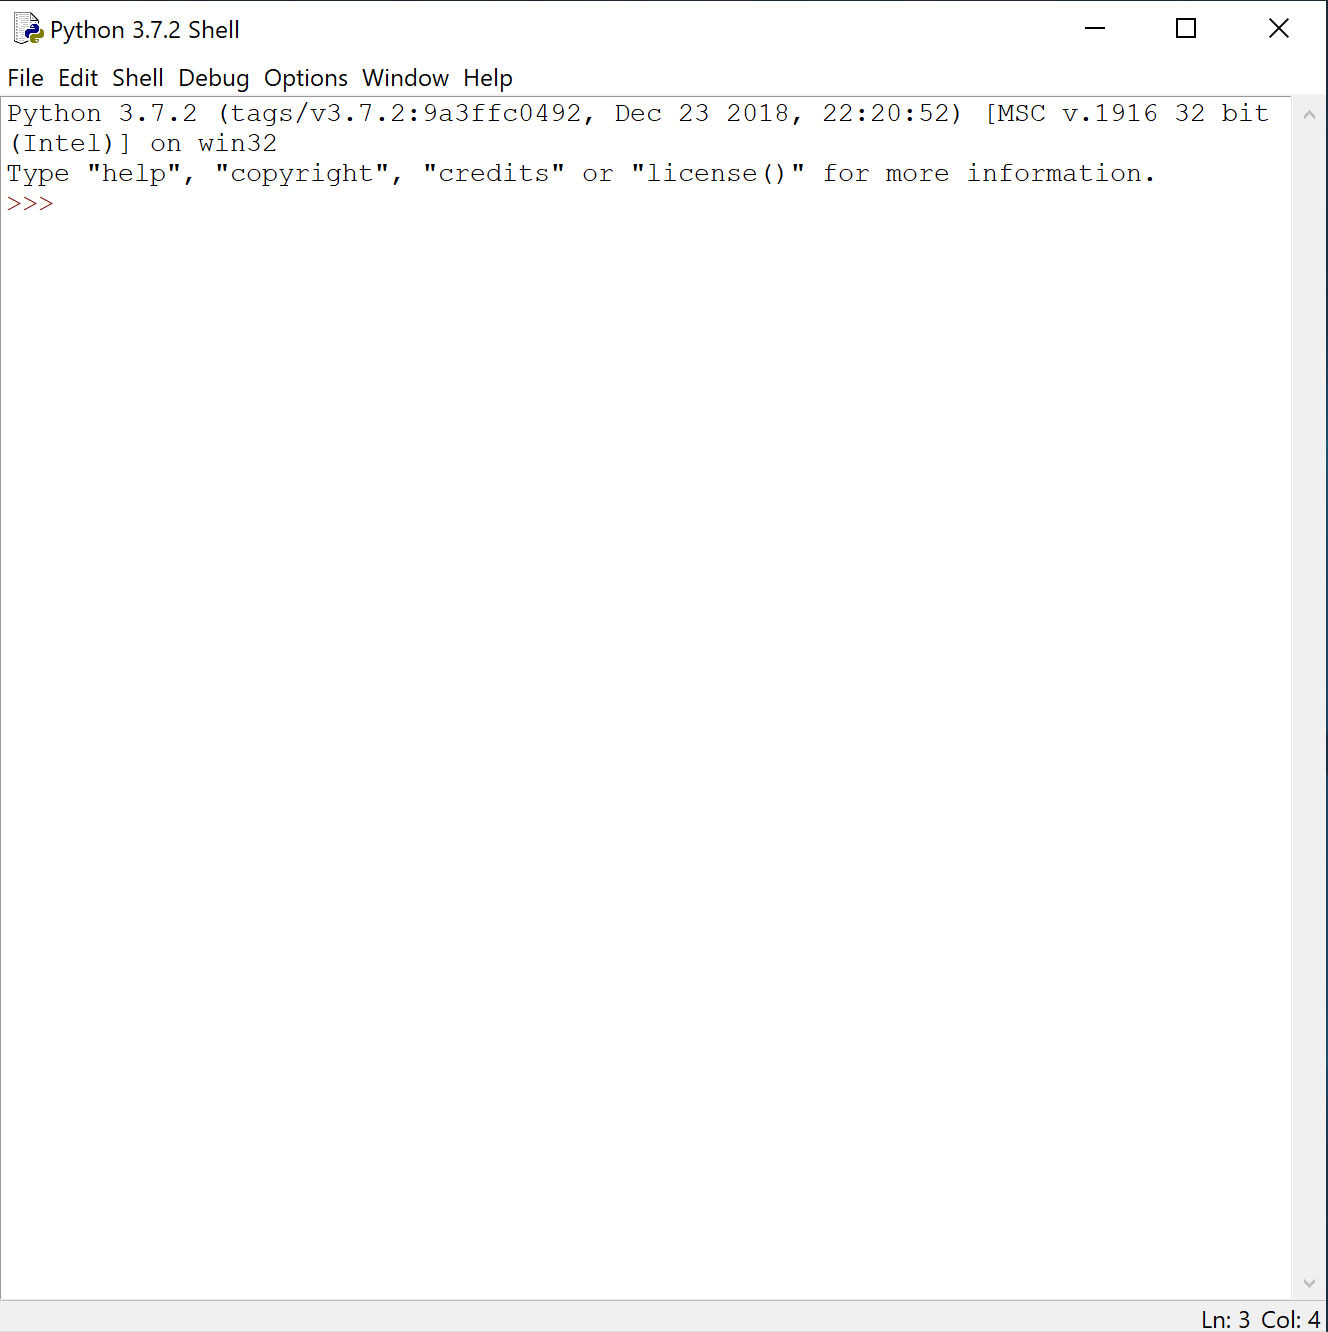
\includegraphics[scale=0.6]{screenshots/idlewin.png}
\end{myfigure}

Using the Option menu, I was able to change the font face to something nicer (I changed it to \href{Fira Code}{https://www.fontsquirrel.com/fonts/fira-code}, the same font used for code examples in these notes) and the font size to something more readable, as you see in Figure \ref{fig:idlewin-hw} on Page \pageref{fig:idlewin-hw}.

\begin{myfigure}[label=fig:idlewin-hw]{IDLE Running on Windows 10 with the Fira Code Font}
    \centering
    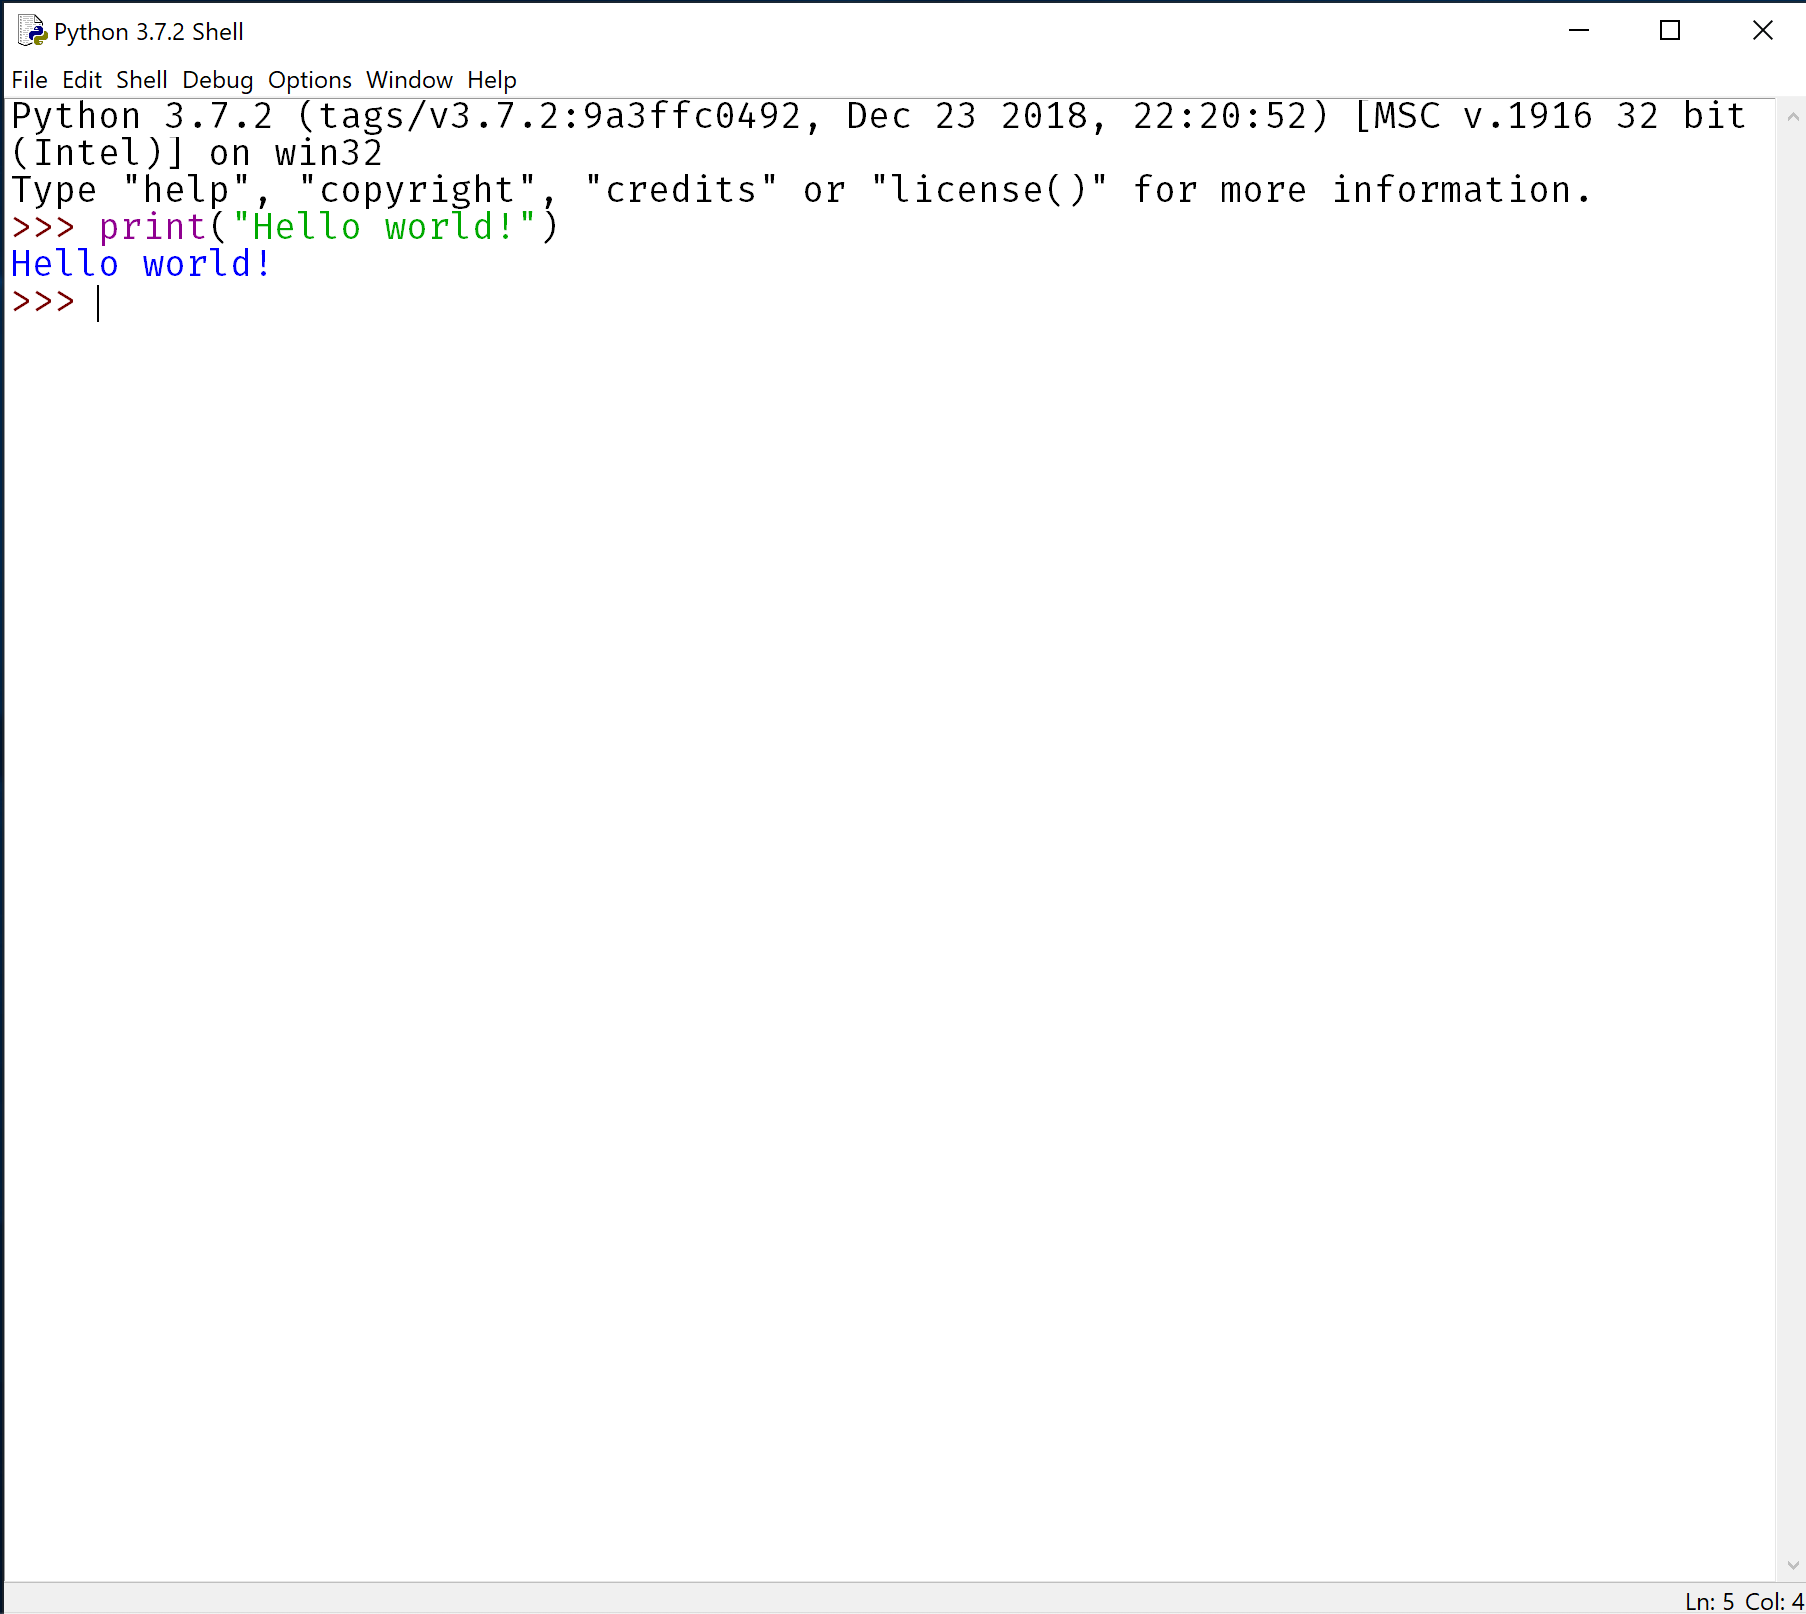
\includegraphics[scale=0.4]{screenshots/idlewin-hw}
\end{myfigure}

\subsection{Mac OS}

There are a couple of ways to install Python and IDLE for Mac OS, but the easiest way is probably the same as in Windows: to download the installation program from \url{https://www.python.org/downloads/} and install.

\subsection{Linux}

On my installation of Ubuntu Linux, I typed the following commands to install IDLE:

\begin{verbatim}
    $ sudo apt update
    $ sudo apt install idle
\end{verbatim}

You could also use the graphical software-installation tool to install IDLE.

Once it's installed, just type \verb-idle- at the command line prompt to open the program.  You should see something like the window in Figure \ref{fig:idlelinux} on Page \pageref{fig:idlelinux}.

\begin{myfigure}[label=fig:idlelinux]{IDLE Running on Ubuntu Linux}
    \centering
    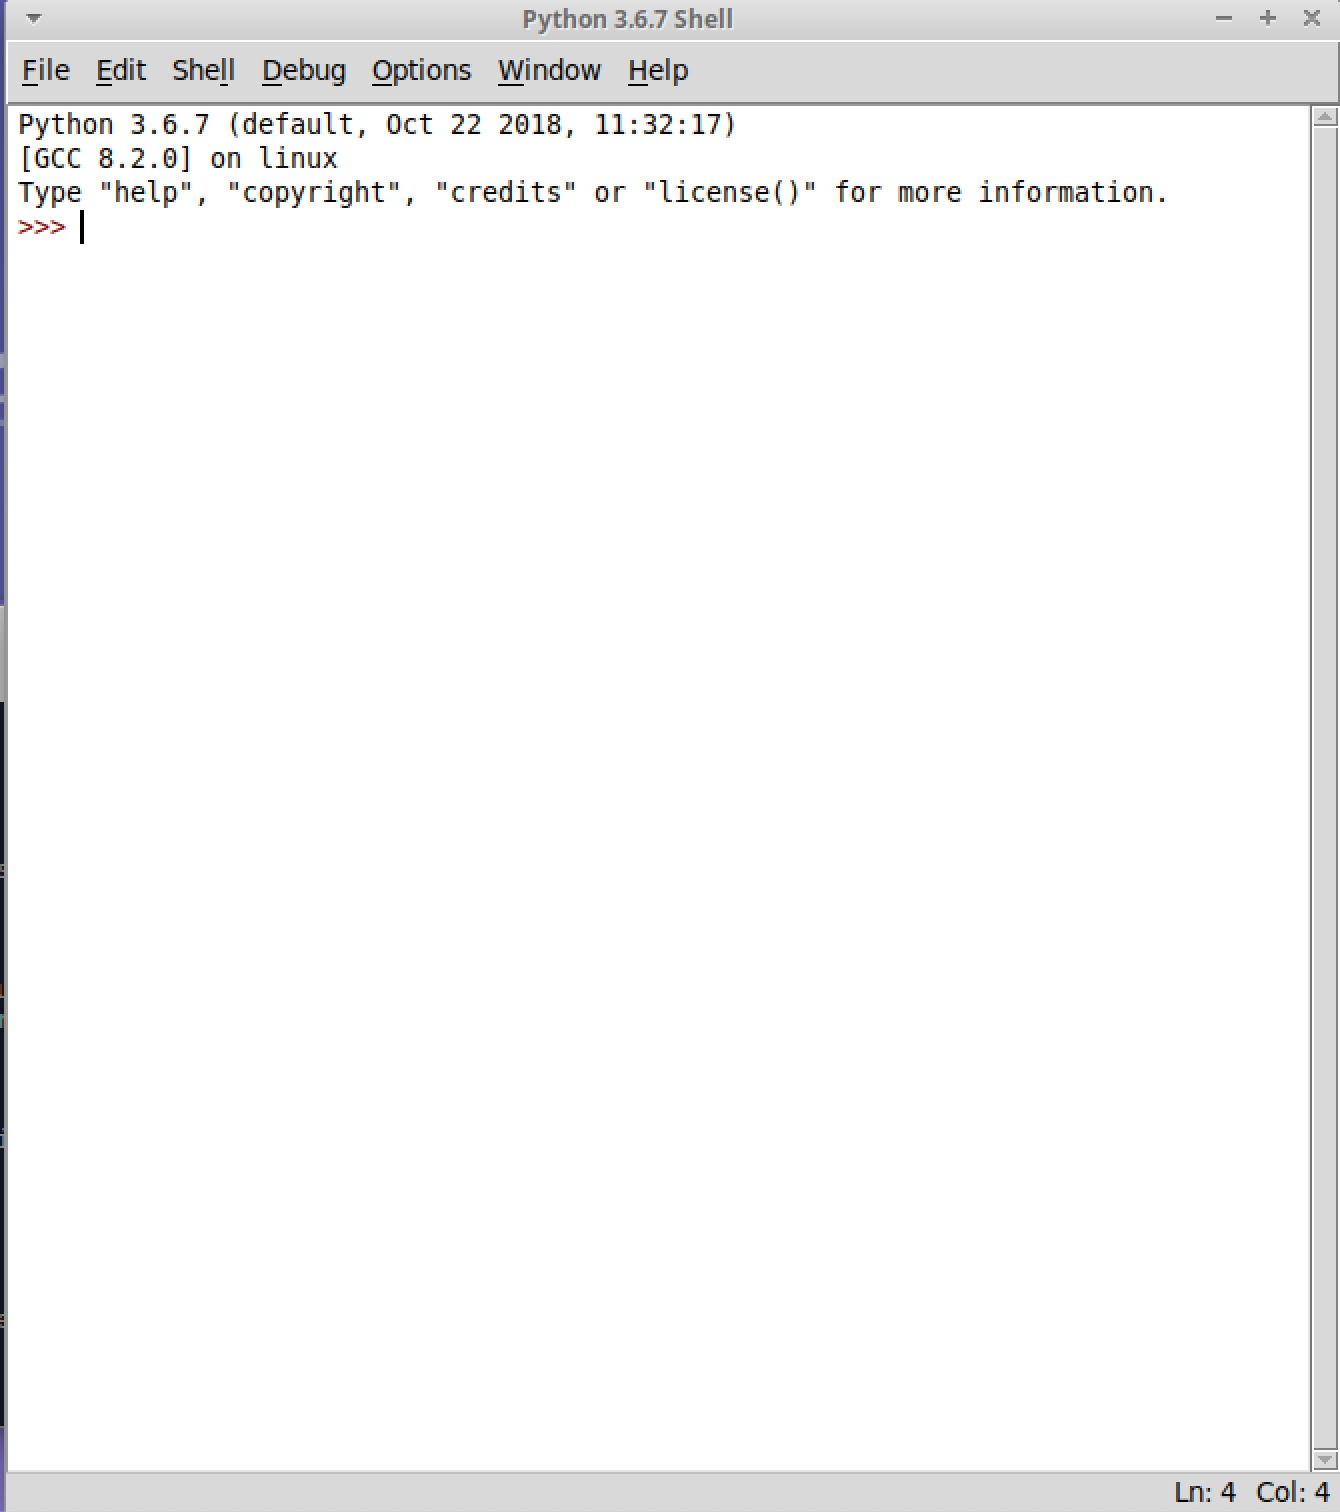
\includegraphics[scale=0.6]{screenshots/idlelinux.png}
\end{myfigure}

It is important that you see the phrase ``Python 3'' at the top of the screen (in this screenshot, it says ``Python 3.6.7'', and that's good).  If it says ``Python 2'' on the first line, then you are running an older version of IDLE -- and therefore an older version of Python -- and things won't work the way you expect.  If this is the case, try running \verb-idle3- instead of just \verb-idle-.  If that doesn't work, try to use \verb-apt- to install \verb-idle3-.
% !TEX root = CSC104LectureNotes.tex

\chapter{Python Keywords}

\index{Reserved words|see {Keywords}}\addindex{Keywords}{Keywords} are words that have a special meaning in Python.  As discussed in XXXXX, we are not allowed to use keywords as identifiers.

This table was copied from this list at W3Schools: \url{https://www.w3schools.com/python/python_ref_keywords.asp}.

Notice that all of these keywords consist completely of lowercase letters except for \texttt{False}, \texttt{True}, and \texttt{None}.

\bigskip

\newcolumntype{K}{%
    >{\raggedleft\ttfamily}p{0.2\textwidth}
}

\topcaption{The Keywords of the Python Language} \label{tab:keywords}

\tablefirsthead{\hline \multicolumn{1}{r}{\textbf{Keyword}} &
    \multicolumn{1}{l}{\textbf{Meaning}} \\ \hline }
    
\tablehead{\multicolumn{2}{c}%
    {{\captionsize\bfseries \tablename\ \thetable{} --
    continued from previous page}} \\
    \hline \multicolumn{1}{r}{\textbf{Keyword}} &
    \multicolumn{1}{l}{\textbf{Meaning}} \\ \hline }

\tabletail{\hline \multicolumn{2}{r}{{\textit{Continued on next page}}} \\}
\tablelasttail{\hline \hline}

\xentrystretch{-0.175}

\begin{xtabular}{K p{.80\textwidth}} 
    and & A logical operator\\
    as & To create an alias\\
    assert & For debugging\\
    break & To break out of a loop\\
    class & To define a class\\
    continue & To continue to the next iteration of a loop\\
    def & To define a function\\
    del & To delete an object\\
    elif & Used in conditional statements, same as else if\\
    else & Used in conditional statements\\
    except & Used with exceptions, what to do when an exception occurs\\
    False & Boolean value, result of comparison operations\\
    finally & Used with exceptions, a block of code that will be executed no matter if there is an exception or not\\
    for & To create a for loop\\
    from & To import specific parts of a module\\
    global & To declare a global variable\\
    if & To make a conditional statement\\
    import & To import a module\\
    in & To check if a value is present in a list, tuple, etc.\\
    is & To test if two variables are equal\\
    lambda & To create an anonymous function\\
    None & Represents a null value\\
    nonlocal & To declare a non-local variable\\
    not & A logical operator\\
    or & A logical operator\\
    pass & A null statement, a statement that will do nothing\\
    raise & To raise an exception\\
    return & To exit a function and return a value\\
    True & Boolean value, result of comparison operations\\
    try & To make a try...except statement\\
    while & To create a while loop\\
    with & Used to simplify exception handling\\
    yield & To end a function, returns a generator\\
\end{xtabular}


\backmatter

\addcontentsline{toc}{chapter}{Index}
\printindex
\end{document}
